\chapter{Structure of proteic complex}

Proteins are biological molecules found in all the living cells.
They are formed of a chain of amino acids \cite{Prot}.
Proteins realize many functions within the living cells.
They can have an enzymatic, structural role, they allow the mobility of molecules,
 the regulation of the genetic expression or to pass on cellular signals.
The protein chains forming the proteins are synthesized in the cell.
 The genetic material of the cell determines the order of the amino acids.

 The proteins have a structure in three dimensions which allows them
 to realize their biological function. Proteins can interact together to
 carry out some biological functions. These interactions form protein
  complexes. The structures of the proteins and their interactions are particularly used
   in medicinal chemistry.
 The study of surfaces and available spaces can guide the research for new medicine.
  Crystallography is used to study the structure of proteins at
   the atomic scale. It is based on the physical phenomenon of diffraction
    of the electromagnetic waves (X-rays).

The data from a protein that we can us is stored in \textit{.pdb} files
(see figure\ref{fig:: pdb_file}). These files, the reading and the interpretation
 of the data they contain, are essential to the observation of proteins.
 Indeed, every line, excepted the first one, corresponds to an atom of protein
 being studied.
These lines contain information such as the chain to which the atom belongs,
its amino acid or its address and coordinates in space ($\si{\angstrom}$).

\begin{figure}[ht]
  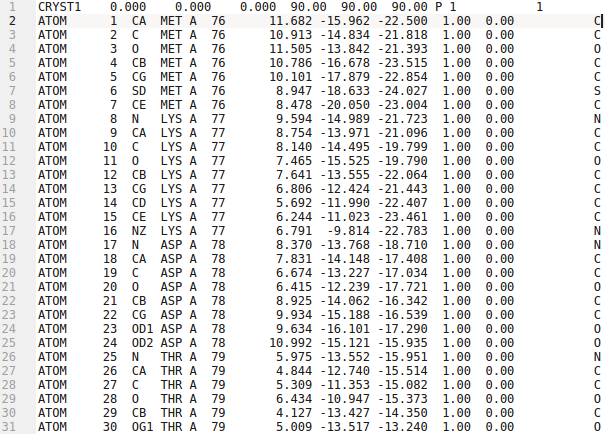
\includegraphics[width=\textwidth]{figures/pdb_example.png}
  \caption{Example of a .pdb file}
  \label{fig::pdb_file}
\end{figure}

During the project, we will consider that atoms are points of the space of identical masses.
First, the address and coordinates of atoms will be extracted.
The point cloud obtained constitutes the basis on which the
method of determination of the interface is going to be based. It is thus crucial
to obtain from the file \textit{.pdb } a set of valid and usable data
for the program to be implemented. We will also see that other information, such as
 the chain (A or B, column 5 of the figure \ref{fig:: pdb_file}),
  plays a leading role in the running of the program. Thus the objective is
   to extract a coherent point cloud (modelling the complex), to apply
    the triangulation of Delaunay.
